\graphicspath{{./figures}}

\section{PocketQube Unit}
\subsection{Circuit Design}
To design the PocketQube PCB, since no development boards were used, the Arduino Nano schematic in \cite{design-arduinoNano} was consulted as a reference design. It was decided to simply expose the relevant pins needed to flash the MCU, instead of integrating a USB connection directly, however this could be added for future iterations. The final circuit schematic can be found in Appendix \ref{sec:appendix_pq_schematic}.

\subsection{Power}
The maximum power consumptions of the on-board components is found in Table \ref{tab:pqunit_component_consumption}. Since the power is provided by an external source, this is simply calculator as a figure of merit, and to allow for sizing of a battery for development purposes. Again, maximum current values are listed. A total maximum power consumption of around 600 mW is calculated.
\begin{table}[!htb]
  \centering
  \renewcommand{\arraystretch}{1.2}
  \begin{tabular}{ |c|c|c| }
  \hline
  \textbf{Component}        & \textbf{Current}        & \textbf{Power (@ 3V3)}      \\ \hline 
  ATmega328                 & 0.2 mA                  & 0.66 mW                     \\ \hline 
  RA-02                     & 100 mA                  & 330 mW                      \\ \hline 
  ATGM332D-5N               & 25 mA                   & 82.5 mW                     \\ \hline
  SN75179B                  & 57 mA                   & 188 mW                      \\ \hline
  \end{tabular}
  \caption{PocketQube Unit Component Power Consumption}
  \label{tab:pqunit_component_consumption}
\end{table}


\subsection{PCB Design}
\begin{figure}[!htb]
  \centering
  \begin{minipage}{.43\textwidth}
    \centering
    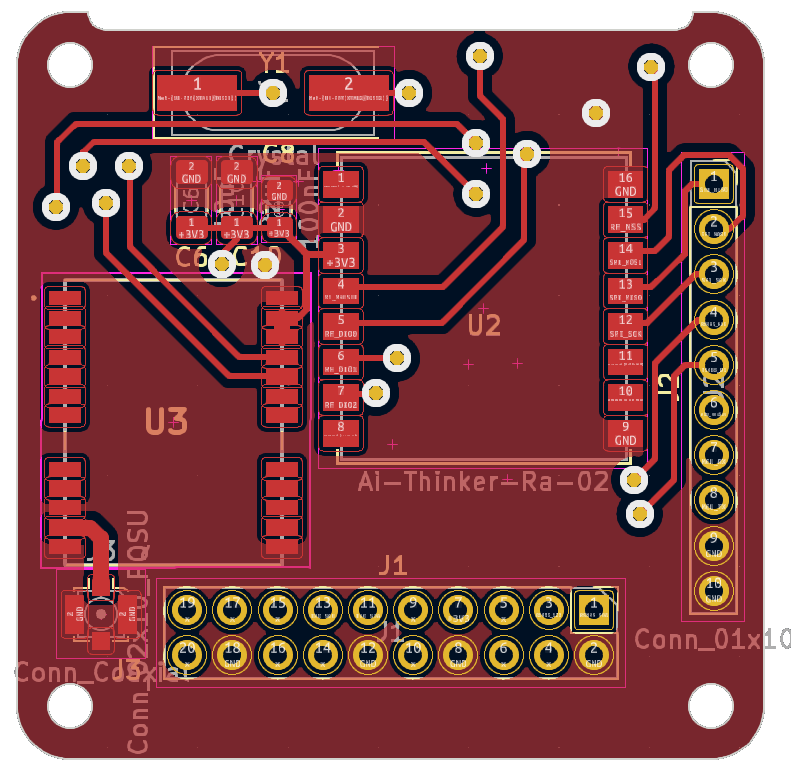
\includegraphics[width=.9\linewidth]{pqunit_pcb_design_front}
    \captionof{figure}{PocketQube Unit PCB Design (Front)}
    \label{fig:pqunit_pcb_design_front}
  \end{minipage}
  \begin{minipage}{.43\textwidth}
    \centering
    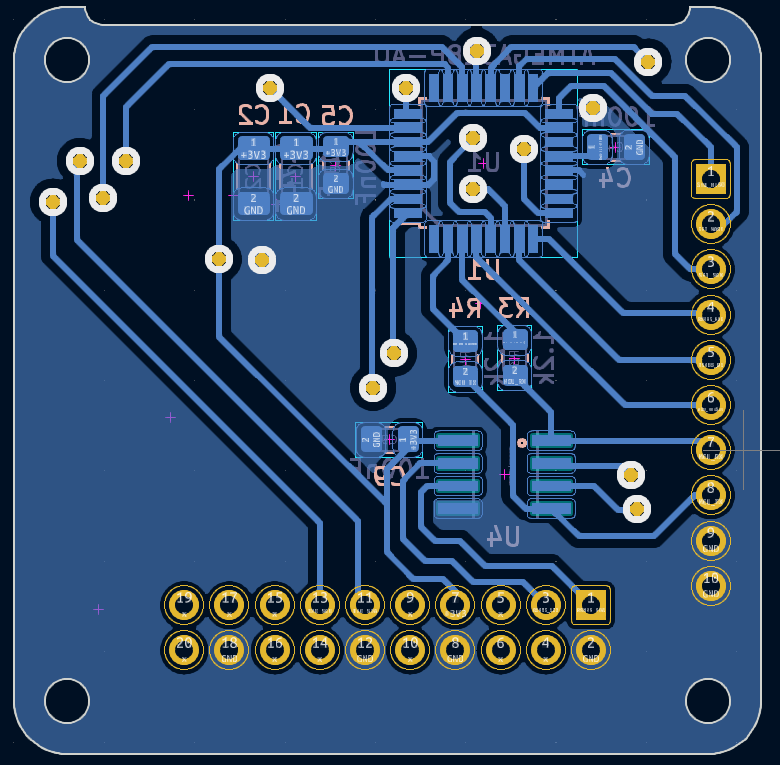
\includegraphics[width=.9\linewidth]{pqunit_pcb_design_back}
    \captionof{figure}{PocketQube Unit PCB Design (Back)}
    \label{fig:pqunit_pcb_design_back}
  \end{minipage}
  \end{figure}

The final PCB was designed to conform to the PocketQube standard, as shown in Figures \ref{fig:pqunit_pcb_design_front} and \ref{fig:pqunit_pcb_design_back}.